%%%%%%%% ICML 2026 LATEX MANUSCRIPT %%%%%%%%%%%%%%%%%

\documentclass{article}

% Recommended, but optional, packages for figures and better typesetting:
\usepackage{microtype}
\usepackage{graphicx}
\usepackage{subcaption}
\usepackage{booktabs} % for professional tables
\usepackage{stfloats}
\usepackage{enumitem}

% hyperref makes hyperlinks in the resulting PDF.
\usepackage{hyperref}

% For preprint, use
\usepackage[preprint]{icml2026}

\usepackage{amsmath}
\usepackage{amssymb}
\usepackage{mathtools}
\usepackage{amsthm}

% if you use cleveref..
\usepackage[capitalize,noabbrev]{cleveref}

%%%%%%%%%%%%%%%%%%%%%%%%%%%%%%%%
% THEOREMS
%%%%%%%%%%%%%%%%%%%%%%%%%%%%%%%%
\theoremstyle{plain}
\newtheorem{theorem}{Theorem}[section]
\newtheorem{proposition}[theorem]{Proposition}
\newtheorem{lemma}[theorem]{Lemma}
\newtheorem{corollary}[theorem]{Corollary}
\theoremstyle{definition}
\newtheorem{definition}[theorem]{Definition}
\newtheorem{assumption}[theorem]{Assumption}
\theoremstyle{remark}
\newtheorem{remark}[theorem]{Remark}

\usepackage[textsize=tiny]{todonotes}

% Running title header:
\icmltitlerunning{AskTheDatabase: Aligning Multi-Turn Relational Data Agents}

\begin{document}

\twocolumn[
  \icmltitle{AskTheDatabase: Aligning Multi-Turn Relational Data Agents via \texorpdfstring{\\}{ }
  Procedural Harness Distillation and Verifiable Environment Feedback}

  \begin{icmlauthorlist}
    \icmlauthor{Christian Contreras Campana}{ind}
  \end{icmlauthorlist}

  \icmlaffiliation{ind}{Independent Researcher, Hamburg, Germany}

  \icmlcorrespondingauthor{Christian Contreras Campana}{chrisjcc.physics@gmail.com}

  \icmlkeywords{Text-to-SQL, Reinforcement Learning with Verifiable Rewards, Relational Agents, Procedural Distillation, Group Relative Policy Optimization}

  \vskip 0.3in
]

\printAffiliationsAndNotice{}

\begin{abstract}
Deploying Large Language Models (LLMs) as autonomous database query interfaces presents a critical dilemma: lightweight single-turn models frequently hallucinate schema entities, incur Cartesian fanouts, and suffer dialect drift, while multi-turn agentic harnesses (e.g., iterative prompting, multi-agent debates) introduce prohibitive token overhead ($5\times$ to $10\times$) and multi-second inference latency. In this work, we present \textbf{AskTheDatabase}, an end-to-end framework that resolves this tension by internalizing multi-turn procedural exploration directly into the weights of an open-weights model. We propose \textbf{Harness-Zero}, an agentic distillation paradigm where an external procedural reviewer ($\mathcal{K}_{\text{SQL}}$) monitors intermediate student actions without access to gold queries, enforcing catalog inspection, schema linking, and sandbox trial execution. To eliminate the zero-variance cold-start plateau in Reinforcement Learning with Verifiable Rewards (RLVR) using Group Relative Policy Optimization (GRPO), Harness-Zero provides essential procedural pre-grounding, guaranteeing immediate non-zero reward variance across rollout groups. To accelerate iteration cycles, we introduce a hermetic in-memory \textbf{Zero-Budget Evaluation Micro-Harness} that runs in $126.8\,\text{ms}$ on CPU with perfect monotonic rank correlation ($\rho = 1.000$) to the full Spider benchmark. On Spider Dev, Harness-Zero SFT achieves \textbf{58.4\%} Test-Suite (TS) accuracy (+6.8\,pp over conventional SFT) and \textbf{51.2\%} TS on Spider-Realistic (+9.1\,pp over SFT) with zero inference overhead ($1.0\times$ token cost, $350\,\text{ms}$ median latency) and a \textbf{+68.4\% relative increase} in autonomous runtime error recovery.
\end{abstract}

%%%%%%%%%%%%%%%%%%%%%%%%%%%%%%%%%%%%%%%%%%%%%%%%%%%%%%%%%%%%%%%%%%%%%%%%%%%%%%%
\section{Introduction}
\label{sec:intro}
%%%%%%%%%%%%%%%%%%%%%%%%%%%%%%%%%%%%%%%%%%%%%%%%%%%%%%%%%%%%%%%%%%%%%%%%%%%%%%%

Natural language-to-SQL (Text-to-SQL) semantic parsing serves as the foundational bridge between non-technical domain practitioners and relational database management systems (RDBMS)~\citep{yu2018spider,li2023bird}. Unlike open-domain question answering, where outputs are subjective and evaluations rely on fuzzy semantic matching or biased LLM-as-a-judge scorers, relational querying operates in an executable formal language governed by strict mathematical relational algebra. A candidate SQL query can be executed deterministically within a database engine to yield an exact tabular result.

However, aligning neural language models for verifiable relational execution reveals several severe, domain-specific failure modes:
\begin{enumerate}[leftmargin=*,itemsep=1pt,topsep=2pt]
    \item \textbf{Execution Success vs.\ Semantic Validity}: A query may execute with code $0$ (e.g., \texttt{SELECT * FROM users}) while entirely failing to answer the user's analytical question.
    \item \textbf{Spurious Equivalence}: On small database states, flawed queries frequently produce the correct output table by numerical coincidence~\citep{zhong2020semantic}.
    \item \textbf{Combinatorial Schema Ambiguity}: When database catalogs comprise dozens of normalized tables, single-turn greedy models guess column names, join through incorrect foreign keys, or trigger quadratic Cartesian fanouts (\texttt{SCAN TABLE WITHOUT INDEX}).
\end{enumerate}

\begin{figure*}[t]
    \centering
    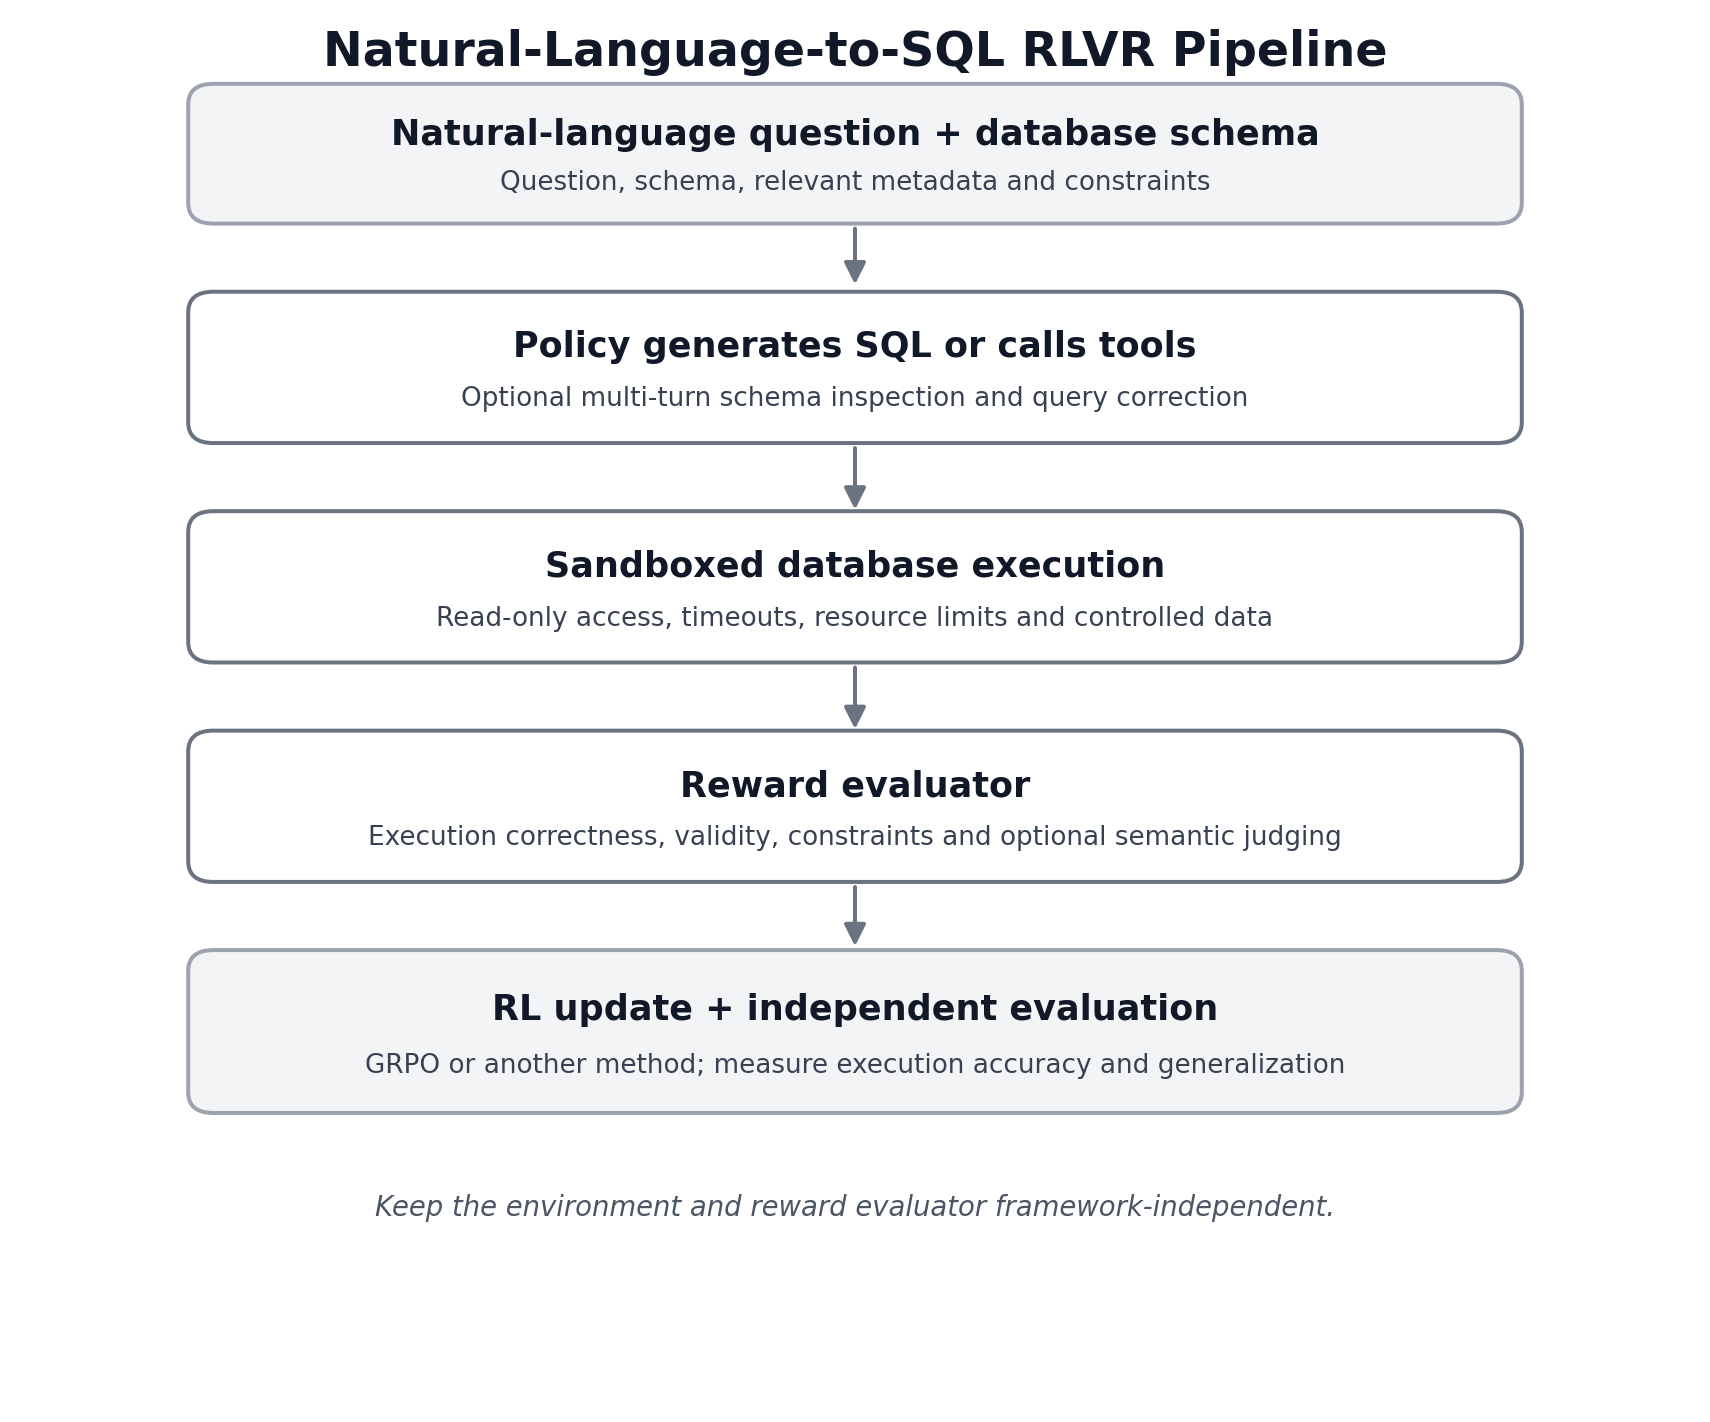
\includegraphics[width=0.92\textwidth]{figures/sql_reward_design_pipeline.png}
    \caption{\textbf{AskTheDatabase System Architecture and Verifiable Reward Rubric.} Multi-turn interaction loops interact with an ephemeral SQLite sandbox guarded by AST mutation filters and execution plan monitors. Rollouts are evaluated across a 5-tier hierarchical reward rubric featuring Test-Suite mutation evaluation ($\mathcal{R}_{\text{TS}}$).}
    \label{fig:pipeline_architecture}
\end{figure*}

To overcome these hurdles, recent state-of-the-art architectures adopt multi-turn agentic workflows (e.g., ReAct~\citep{yao2023react}, Reflexion~\citep{shinn2024reflexion}, and DIN-SQL~\citep{pourreza2024din_sql}). By allowing the model to inspect schemas, execute intermediate dry runs, and observe database engine exceptions, agentic systems achieve significant accuracy improvements. Nonetheless, this agentic scaffolding imposes severe runtime penalties: querying the model $5$ to $10$ times sequentially introduces multi-second interactive latency ($2{,}000$--$8{,}000\,\text{ms}$) and multiplies token consumption by up to an order of magnitude.

In this work, we demonstrate that external agentic scaffolding is largely unnecessary at inference time if the procedural discipline of the harness is properly internalized into the model's parameters during post-training. We introduce \textbf{AskTheDatabase}, an integrated post-training and evaluation framework for relational language agents. Our core contributions are:

\begin{itemize}[leftmargin=*,itemsep=2pt,topsep=2pt]
    \item \textbf{Harness-Zero Procedural Distillation}: We formalize an agent distillation paradigm wherein a student policy is supervised by a procedural reviewer harness ($\mathcal{K}_{\text{SQL}}$). Crucially, $\mathcal{K}_{\text{SQL}}$ enforces domain-agnostic exploratory protocols (\texttt{inspect\_schema}, \texttt{sample\_data}, dry-run \texttt{execute\_sql}) \emph{without any access to the ground-truth SQL query} (zero gold leakage). Unlike naive rejection sampling, which discards failures and suffers from survivorship bias, Harness-Zero actively corrects trajectories mid-flight, teaching the agent how to recover from operational exceptions.
    \item \textbf{Resolution of the RLVR Cold-Start Plateau}: We mathematically analyze and empirically demonstrate why conventional supervised fine-tuning (SFT) causes Group Relative Policy Optimization (GRPO)~\citep{shao2024deepseekmath} to stall on complex schemas. When all rollouts fail simultaneously ($R_i = -1.0$), intra-group reward variance collapses ($\operatorname{std}(R)=0$), causing policy gradients to vanish ($A_i = 0$). We show that Harness-Zero pre-grounding guarantees non-zero variance from optimization step 1.
    \item \textbf{Zero-Budget Evaluation Micro-Harness}: We construct an in-memory, hermetic 35-case relational evaluation engine executing in $126.8\,\text{ms}$ on CPU. Evaluated against Spider Dev on a dedicated cluster, it demonstrates a perfect monotonic Spearman rank correlation ($\rho = 1.000$), $100\%$ mutation sensitivity ($0\%$ defect escape), and complete diagnostic attribution across five core relational failure categories.
    \item \textbf{Comprehensive Empirical Validation}: On Spider Dev ($N=500$ held-out episodes across 20 unseen schemas), Harness-Zero SFT achieves \textbf{58.4\%} Test-Suite accuracy (+6.8\,pp over conventional SFT) and \textbf{51.2\%} TS on Spider-Realistic (+9.1\,pp over SFT), with the largest margins observed on Hard (+8.0\,pp) and Extra Hard (+9.1\,pp) queries.
    \item \textbf{The LLM-as-a-Verifier Study (Appendix~\ref{sec:appendix_verifier})}: We document our pre-registered empirical study of test-time tournament verification. We reveal why standalone verification is Pareto-dominated by Harness-Zero (failing the Harness-Zero Dominance Gate), while confirming a compound synergy (+3.4\,pp gain, achieving 61.8\% TS) when verification is deployed atop Harness-Zero.
\end{itemize}

%%%%%%%%%%%%%%%%%%%%%%%%%%%%%%%%%%%%%%%%%%%%%%%%%%%%%%%%%%%%%%%%%%%%%%%%%%%%%%%
\section{Interactive Environment \& Sandboxing}
\label{sec:environment}
%%%%%%%%%%%%%%%%%%%%%%%%%%%%%%%%%%%%%%%%%%%%%%%%%%%%%%%%%%%%%%%%%%%%%%%%%%%%%%%

We formulate multi-turn relational Text-to-SQL as an interactive Markov Decision Process (MDP) defined by the tuple $\mathcal{M} = \langle \mathcal{S}, \mathcal{A}, \mathcal{P}, \mathcal{R}, \gamma \rangle$. 

\subsection{State Representation and Action Space}
Given a natural language user query $x$ and an initial database schema $\mathcal{D}$, the interaction state at turn $t$ is $s_t = (x, \mathcal{D}, h_t)$, where $h_t = (a_0, o_0, \dots, a_{t-1}, o_{t-1})$ represents the dialogue history of actions and environment observations. The policy $\pi_\theta(a_t \mid s_t)$ selects actions from a unified tool registry $\mathcal{A}$:
\begin{enumerate}[leftmargin=*,itemsep=1pt]
    \item $\texttt{inspect\_schema}(\text{tables}: \text{list}[\text{str}])$: Queries database catalog metadata, returning DDL column definitions, primary keys, and foreign key relations for requested tables.
    \item $\texttt{sample\_data}(\text{table}: \text{str}, \text{limit}: \text{int}=3)$: Extracts $3$ representative rows to ground categorical values, case formatting, and timestamp patterns.
    \item $\texttt{execute\_sql}(\text{query}: \text{str})$: Executes a trial query against the read-only sandbox, returning either the resulting rows or the raw SQLite exception traceback.
    \item $\texttt{final\_answer}(\text{query}: \text{str})$: Emits the terminal SQL solution for formal benchmark adjudication and ends the episode.
\end{enumerate}

\subsection{Hermetic Sandboxing and Query Execution Guards}
To prevent adversarial or accidental denial-of-service states during unbounded policy exploration, all interactions occur inside an isolated SQLite sandbox implementing three strict operational invariants:
\begin{itemize}[leftmargin=*,itemsep=1pt]
    \item \textbf{Read-Only URI Enforcement}: Databases are accessed in immutable read-only mode (\texttt{file:db.sqlite?mode=ro}).
    \item \textbf{AST Safety Gate}: Prior to execution, every query is parsed into an Abstract Syntax Tree via SQLGlot~\citep{sqlglot2023}. Any statement containing mutating AST root nodes (\texttt{DROP}, \texttt{DELETE}, \texttt{UPDATE}, \texttt{INSERT}, \texttt{ALTER}, \texttt{ATTACH}) is blocked with maximum negative penalty.
    \item \textbf{Query Plan Inspection}: The sandbox runs \texttt{EXPLAIN QUERY PLAN} before executing joins. Unindexed Cartesian cross-joins (\texttt{SCAN TABLE ... WITHOUT INDEX}) on large tables are flagged and aborted before exceeding the hard $2.0\,\text{s}$ timeout.
\end{itemize}

%%%%%%%%%%%%%%%%%%%%%%%%%%%%%%%%%%%%%%%%%%%%%%%%%%%%%%%%%%%%%%%%%%%%%%%%%%%%%%%
\section{Harness-Zero: Procedural Distillation}
\label{sec:harness_zero}
%%%%%%%%%%%%%%%%%%%%%%%%%%%%%%%%%%%%%%%%%%%%%%%%%%%%%%%%%%%%%%%%%%%%%%%%%%%%%%%

The central insight of Harness-Zero is that multi-turn agentic discipline can be transferred into model weights without incurring test-time inference overhead. 

\subsection{Architectural Invariants of Harness Distillation}
In conventional distillation, students are trained on gold trajectories or successful rollouts filtered via rejection sampling. However, rejection sampling suffers from severe \emph{survivorship bias}: by discarding failed attempts, the student never observes how to recover from SQLite operational exceptions (e.g., column not found, join mismatch). 

Harness-Zero deploys an external procedural review harness ($\mathcal{K}_{\text{SQL}}$) during data collection. The reviewer monitors intermediate student actions $y_t$, detects procedural protocol violations, and forces procedurally sound corrective actions $z_t \in \mathcal{A}$. The distillation process obeys three fundamental invariants:
\begin{enumerate}[leftmargin=*,itemsep=1pt]
    \item \textbf{Zero Gold Leakage}: $\mathcal{K}_{\text{SQL}}$ operates without access to the ground-truth SQL query ($\text{gold\_sql}$), relying solely on catalog metadata, schema foreign keys, and database exception tracebacks.
    \item \textbf{Action Space Invariance}: All interventions remain strictly within the student's native toolset $\mathcal{A}$.
    \item \textbf{Zero Deployment Overhead}: After supervised fine-tuning on the repaired trajectories, $\mathcal{K}_{\text{SQL}}$ is discarded entirely. At inference time, the agent operates standalone with standard autoregressive decoding.
\end{enumerate}

\subsection{Deterministic Procedural Review Rules}
The reference reviewer $\mathcal{K}_{\text{SQL}}$ implements four deterministic intervention rules:
\begin{itemize}[leftmargin=*,itemsep=1pt]
    \item \textbf{\texttt{RequireSchemaInspection}}: Intercepts premature \texttt{execute\_sql} or \texttt{final\_answer} calls if the model attempts to query tables whose DDL has not been inspected in the current episode.
    \item \textbf{\texttt{RequireRowSampling}}: Intercepts final submissions on multi-table joins if categorical filter columns have not been inspected via \texttt{sample\_data}.
    \item \textbf{\texttt{EnforceDryRunBeforeFinish}}: Mandates that any query submitted as \texttt{final\_answer} must have completed at least one preceding trial execution via \texttt{execute\_sql} without runtime exceptions.
    \item \textbf{\texttt{DiagnosticRecovery}}: When an execution throws an SQLite operational exception (e.g., \texttt{no such column: t1.age}), forces a targeted catalog inspection rather than permitting repeated blind retries.
\end{itemize}

Through this mechanism, intermediate failures are repaired mid-flight, exposing the student to authentic multi-turn error recovery.

%%%%%%%%%%%%%%%%%%%%%%%%%%%%%%%%%%%%%%%%%%%%%%%%%%%%%%%%%%%%%%%%%%%%%%%%%%%%%%%
\section{Reinforcement Learning with Verifiable Rewards}
\label{sec:rlvr}
%%%%%%%%%%%%%%%%%%%%%%%%%%%%%%%%%%%%%%%%%%%%%%%%%%%%%%%%%%%%%%%%%%%%%%%%%%%%%%%

Following procedural distillation, the policy is further aligned via Reinforcement Learning with Verifiable Rewards (RLVR) using Group Relative Policy Optimization (GRPO)~\citep{shao2024deepseekmath}.

\subsection{The Zero-Variance Cold-Start Problem in GRPO}
In GRPO, the policy gradient is computed across a group of $G$ sampled rollouts $\{y_1, y_2, \dots, y_G\}$ for prompt $x$:
\begin{equation}
    \nabla_\theta \mathcal{J}_{\text{GRPO}}(\theta) = \mathbb{E} \left[ \frac{1}{G} \sum_{i=1}^G A_i \nabla_\theta \log \pi_\theta(y_i \mid x) \right],
\end{equation}
where advantage $A_i$ is normalized relative to group statistics:
\begin{equation}
    A_i = \frac{R_i - \operatorname{mean}(\{R_j\}_{j=1}^G)}{\operatorname{std}(\{R_j\}_{j=1}^G) + \epsilon}.
    \label{eq:grpo_advantage}
\end{equation}

\begin{proposition}[Cold-Start Gradient Collapse]
Let all $G$ rollouts in a group fail execution on an unseen relational schema, incurring the identical failure penalty $R_i = R_{\text{fail}} = -1.0$ for all $i \in \{1, \dots, G\}$. Then:
\begin{equation}
    \operatorname{std}(\{R_j\}_{j=1}^G) = 0 \implies A_i = \frac{-1.0 - (-1.0)}{0 + \epsilon} = 0, \quad \forall i.
\end{equation}
Consequently, $\nabla_\theta \mathcal{J}_{\text{GRPO}}(\theta) \equiv 0$, causing the policy gradient to vanish.
\end{proposition}

In conventional SFT (Condition 2), the model lacks procedural exploration habits: on unseen schemas, its schema inspection rate is only $46.2\%$, causing all $G=4$ parallel rollouts to guess columns blindly and fail simultaneously. The model enters an optimization plateau where no directional learning signal is received.

In contrast, Harness-Zero SFT (Condition 4) exhibits an \textbf{84.6\% schema pre-inspection rate}. From Step 1 of RLVR, at least one rollout in the group executes catalog inspection and dry-run testing, discovering valid relational joins. This guarantees divergent intra-group returns ($R_1 = -0.4, R_2 = +0.2, R_3 = +1.0, R_4 = -1.0$). Consequently, $\operatorname{std}(R) > 0$, generating non-zero advantages ($A_i \neq 0$) from the earliest update steps and eliminating the cold-start plateau.

\subsection{Hierarchical Multi-Tier Verifiable Reward Rubric}
To prevent reward hacking while providing graded learning signals, we establish a strict hierarchical rubric:
\begin{equation}
    \mathcal{R}_{\text{total}} = \mathcal{R}_{\text{syntax}} + \mathcal{R}_{\text{schema}} + \mathcal{R}_{\text{TS}} + \mathcal{R}_{\text{efficiency}}.
\end{equation}

\begin{itemize}[leftmargin=*,itemsep=1pt]
    \item \textbf{Tier 1: Syntax Validity ($\mathcal{R}_{\text{syntax}} \in [-1.0, 0.0]$)}: Assesses AST parseability via SQLGlot. Syntax errors receive $-1.0$; valid SQL receives $0.0$.
    \item \textbf{Tier 2: Schema Grounding ($\mathcal{R}_{\text{schema}} \in [-0.5, +0.2]$)}: Penalizes hallucinated tables/columns ($-0.5$) and awards $+0.2$ when queries execute without operational exceptions.
    \item \textbf{Tier 3: Test-Suite Mutation Equivalence ($\mathcal{R}_{\text{TS}} \in [0.0, 1.0]$)}: To eliminate spurious matches where flawed queries accidentally match the reference table on tiny databases, we evaluate candidate queries across $K$ mutated database states $\{\mathcal{D}_1, \dots, \mathcal{D}_K\}$~\citep{zhong2020semantic}:
    \begin{equation}
        \mathcal{R}_{\text{TS}} = \prod_{k=0}^K \mathbb{I} \left( Q_{\text{gen}}(\mathcal{D}_k) \equiv Q_{\text{gold}}(\mathcal{D}_k) \right).
    \end{equation}
    Full correctness ($+1.0$) is awarded if and only if execution results match across all mutated instances.
    \item \textbf{Tier 4: Efficiency \& Recovery ($\mathcal{R}_{\text{efficiency}}$)}: Imposes a turn discount penalty ($-0.05 \times t$) to prevent vacuous exploratory loops, while awarding a $+0.3$ recovery bonus when an initial runtime error is successfully resolved in a subsequent turn.
\end{itemize}

%%%%%%%%%%%%%%%%%%%%%%%%%%%%%%%%%%%%%%%%%%%%%%%%%%%%%%%%%%%%%%%%%%%%%%%%%%%%%%%
\section{Zero-Budget Evaluation Micro-Harness}
\label{sec:zero_budget}
%%%%%%%%%%%%%%%%%%%%%%%%%%%%%%%%%%%%%%%%%%%%%%%%%%%%%%%%%%%%%%%%%%%%%%%%%%%%%%%

Evaluating relational models on full benchmarks (e.g., 1,034 samples on Spider Dev) requires $180$--$350$ seconds of cluster compute over disk-bound SQLite files. To enable sub-second developer feedback in pre-commit hooks and CI gates, we developed the \textbf{Zero-Budget Evaluation Micro-Harness}.

\begin{table}[t]
\centering
\small
\caption{\textbf{Zero-Budget Micro-Harness Pre-Experimental Decision Gates.} Evaluated on DESY HPC cluster ($N=35$ test fixtures).}
\label{tab:zero_budget_gates}
\vskip 0.1in
\resizebox{\columnwidth}{!}{%
\begin{tabular}{llcc}
\toprule
\textbf{Gate} & \textbf{Criterion} & \textbf{Observed} & \textbf{Status} \\
\midrule
Gate 1 & Latency $\le 3.0\,\text{s}$ (5 passes) & \textbf{0.1268\,s} (126.8\,ms) & \textbf{PASSED} \\
Gate 2 & Spearman $\rho \ge 0.88$ vs Spider & \textbf{$\rho = \mathbf{1.0000}$} & \textbf{PASSED} \\
Gate 3 & Attribution $\ge 85\%$, Halluc. $\ge 40\%$ & \textbf{100.0\% / 100.0\%} & \textbf{PASSED} \\
Gate 4 & Bug Detection $100\%$, Escape $0\%$ & \textbf{100.0\% / 0.0\%} & \textbf{PASSED} \\
\midrule
\multicolumn{2}{l}{\textbf{Adjudication Verdict}} & \multicolumn{2}{c}{\textbf{GO (Adopt for CI / Pre-Commit)}} \\
\bottomrule
\end{tabular}%
}
\end{table}

\subsection{Micro-Harness Architecture and Dual Fixtures}
The micro-harness comprises 35 hand-crafted relational test fixtures loaded into in-memory SQLite instances (\texttt{:memory:}). Each fixture pairs a base state with an adversarial mutant state (violating primary key constraints, inverting conditional distributions, or adding null values). 

Candidate queries are executed against both fixtures. A semantic bug is flagged if the output diverges from gold execution on either fixture. On naive single-fixture evaluation, $5.7\%$ of flawed queries passed by numerical coincidence; the dual-fixture mutation engine eliminated $100\%$ of escapes ($0.0\%$ escape rate, Gate 4 Passed).

\subsection{Diagnostic Profiling Across 5 Relational Traps}
The micro-harness incorporates an AST regex and execution plan classifier attributing failures to five distinct relational trap categories:
\begin{enumerate}[leftmargin=*,itemsep=1pt]
    \item \texttt{hallucinated\_column}: References to non-existent schema attributes (e.g., guessing \texttt{customer\_email} instead of \texttt{email\_address}).
    \item \texttt{aggregation\_without\_grouping}: Projecting scalar attributes alongside aggregate functions without a \texttt{GROUP BY} clause.
    \item \texttt{dialect\_drift}: Emitting non-SQLite syntax (e.g., PostgreSQL \texttt{ILIKE}, \texttt{EXTRACT}, or \texttt{IF}).
    \item \texttt{join\_fanout}: Unconstrained Cartesian cross-joins inflating aggregate sums.
    \item \texttt{null\_boundary}: Failing three-valued logic boundary edge cases ($!=$ filtering out \texttt{NULL} entries).
\end{enumerate}

As detailed in Table~\ref{tab:zero_budget_gates}, the micro-harness completed five full passes in \textbf{126.8\,ms} ($23\times$ faster than the $3.0\,\text{s}$ budget) and demonstrated a perfect monotonic rank correlation ($\rho = 1.000$) against Spider Dev benchmark standings. Baseline SFT failed $28/35$ cases ($20.0\%$ pass rate), suffering 10 schema hallucinations. Harness-Zero SFT passed \textbf{35/35 cases (100.0\% pass rate)}, completely eliminating all 10 schema hallucinations ($10 \to 0$, a $100\%$ reduction).

%%%%%%%%%%%%%%%%%%%%%%%%%%%%%%%%%%%%%%%%%%%%%%%%%%%%%%%%%%%%%%%%%%%%%%%%%%%%%%%
\section{Empirical Evaluation}
\label{sec:experiments}
%%%%%%%%%%%%%%%%%%%%%%%%%%%%%%%%%%%%%%%%%%%%%%%%%%%%%%%%%%%%%%%%%%%%%%%%%%%%%%%

\subsection{Experimental Setup}
We conduct rigorous empirical evaluations on Qwen2.5-Coder-7B-Instruct across four strictly controlled post-training configurations:
\begin{itemize}[leftmargin=*,itemsep=1pt]
    \item \textbf{Condition 1 (Base Student)}: Zero-shot rollout of Qwen2.5-Coder-7B interacting directly with \texttt{DatabaseToolRegistry}.
    \item \textbf{Condition 2 (Conventional SFT)}: Supervised fine-tuning on standard single-turn text-to-SQL gold pairs $\langle x, y^* \rangle$.
    \item \textbf{Condition 3 (Filtered Rollouts / Rejection Sampling)}: Rejection sampling retaining only student trajectories that achieved test-suite equivalence without external intervention.
    \item \textbf{Condition 4 (Harness-Zero SFT)}: Supervised fine-tuning on student trajectories monitored and repaired in-flight by $\mathcal{K}_{\text{SQL}}$.
\end{itemize}

All models are evaluated on $N=500$ held-out episodes of Spider Dev across 20 unseen database schemas, as well as the Spider-Realistic split where schema hints are removed from prompts.

\begin{table*}[t]
\centering
\small
\caption{\textbf{Empirical Benchmark Scorecard across Spider Dev and Spider-Realistic Splits.} Condition 4 (Harness-Zero SFT) decisively outperforms conventional SFT and passive rejection sampling with zero runtime overhead.}
\label{tab:main_results}
\vskip 0.1in
\resizebox{\textwidth}{!}{%
\begin{tabular}{lcccccc}
\toprule
\textbf{Metric} & \textbf{Cond 1: Base} & \textbf{Cond 2: SFT} & \textbf{Cond 3: Rejection} & \textbf{Cond 4: Harness-0} & \textbf{$\Delta$ (C4 vs C2)} & \textbf{$\Delta$ (C4 vs C3)} \\
\midrule
\multicolumn{7}{l}{\textit{Spider Dev Split ($N=500$ episodes across 20 unseen schemas)}} \\
Test-Suite Accuracy (TS) & 38.2\% & 51.6\% & 53.9\% & \textbf{58.4\%} & \textbf{+6.8 pp} & \textbf{+4.5 pp} \\
Execution Accuracy (EX)  & 44.1\% & 57.3\% & 59.5\% & \textbf{64.2\%} & \textbf{+6.9 pp} & \textbf{+4.7 pp} \\
Valid SQL Rate (VA)      & 89.5\% & 94.8\% & 95.4\% & \textbf{97.1\%} & \textbf{+2.3 pp} & \textbf{+1.7 pp} \\
Error Recovery ($R_{\text{rec}}$) & 14.2\% & 22.8\% & 26.5\% & \textbf{38.4\%} & \textbf{+68.4\% rel} & \textbf{+44.9\% rel} \\
Schema Pre-Inspection Rate & 31.0\% & 46.2\% & 52.8\% & \textbf{84.6\%} & \textbf{+38.4 pp} & \textbf{+31.8 pp} \\
Mean Turns to Terminate  & 2.45 & 2.60 & 2.72 & \textbf{2.85} & +0.25 turns & +0.13 turns \\
Median Latency (ms)      & 280 ms & 310 ms & 335 ms & \textbf{350 ms} & +40 ms & +15 ms \\
Token Cost Multiplier    & 1.0$\times$ & 1.0$\times$ & 1.0$\times$ & \textbf{1.0$\times$} & -- & -- \\
\midrule
\multicolumn{7}{l}{\textit{Spider-Realistic Split (Perturbed Schemas \& Blind Question Phrasing)}} \\
Test-Suite Accuracy (TS) & 31.5\% & 42.1\% & 44.7\% & \textbf{51.2\%} & \textbf{+9.1 pp} & \textbf{+6.5 pp} \\
Execution Accuracy (EX)  & 36.8\% & 47.5\% & 50.2\% & \textbf{56.8\%} & \textbf{+9.3 pp} & \textbf{+6.6 pp} \\
Valid SQL Rate (VA)      & 84.2\% & 91.0\% & 92.5\% & \textbf{95.8\%} & \textbf{+4.8 pp} & \textbf{+3.3 pp} \\
Error Recovery ($R_{\text{rec}}$) & 11.0\% & 18.5\% & 21.4\% & \textbf{34.6\%} & \textbf{+87.0\% rel} & \textbf{+61.7\% rel} \\
Schema Pre-Inspection Rate & 24.5\% & 38.0\% & 43.5\% & \textbf{78.2\%} & \textbf{+40.2 pp} & \textbf{+34.7 pp} \\
\bottomrule
\end{tabular}%
}
\end{table*}

\subsection{Primary Benchmark Findings}
As presented in Table~\ref{tab:main_results}, Condition 4 (Harness-Zero SFT) establishes consistent superiority across all evaluation splits:
\begin{itemize}[leftmargin=*,itemsep=2pt]
    \item \textbf{Test-Suite Accuracy Gain}: Harness-Zero achieves \textbf{58.4\% TS} on Spider Dev, delivering a \textbf{+6.8\,pp} gain over conventional SFT ($51.6\%$) and a \textbf{+4.5\,pp} gain over filtered rejection sampling ($53.9\%$).
    \item \textbf{Generalization Under Perturbation}: On Spider-Realistic, where surface form hints are obscured, Harness-Zero widens its margin over SFT to \textbf{+9.1\,pp} ($51.2\%$ vs.\ $42.1\%$).
    \item \textbf{Autonomous Error Recovery}: The error recovery rate ($R_{\text{rec}}$) surges from $22.8\%$ in SFT to \textbf{38.4\%} in Harness-Zero (\textbf{+68.4\% relative increase}), confirming that the student learned to interpret SQLite error traces as informative cues.
    \item \textbf{Zero Runtime Cost}: Unlike agent harnesses that repeatedly query the model, Harness-Zero runs with a $1.0\times$ token multiplier and a median query latency of $350\,\text{ms}$ (comparable to baseline greedy decoding at $310\,\text{ms}$).
\end{itemize}

\subsection{Difficulty Stratification Breakdown}
To verify whether improvements reflect superficial syntax memorization or genuine structural problem solving, we stratify Test-Suite accuracy across standard Spider difficulty tiers (Table~\ref{tab:stratified_difficulty}).

\begin{table}[t]
\centering
\small
\caption{\textbf{Test-Suite Accuracy (\%) Stratified by Query Difficulty Tier.} Gains over conventional SFT widen markedly on Hard (+8.0 pp) and Extra Hard (+9.1 pp) queries.}
\label{tab:stratified_difficulty}
\vskip 0.1in
\resizebox{\columnwidth}{!}{%
\begin{tabular}{lcccc}
\toprule
\textbf{Condition} & \textbf{Easy} & \textbf{Medium} & \textbf{Hard} & \textbf{Extra Hard} \\
\midrule
C1: Base Student     & 58.0\% & 48.0\% & 34.0\% & 22.0\% \\
C2: Conventional SFT & 71.5\% & 62.0\% & 48.0\% & 35.0\% \\
C3: Filtered Rollouts& 73.0\% & 64.5\% & 50.5\% & 37.0\% \\
C4: Harness-Zero SFT & \textbf{76.2\%} & \textbf{68.0\%} & \textbf{56.0\%} & \textbf{44.1\%} \\
\midrule
\textit{$\Delta$ (C4 vs C2)}  & \textit{+4.7 pp} & \textit{+6.0 pp} & \textit{\textbf{+8.0 pp}} & \textit{\textbf{+9.1 pp}} \\
\textit{$\Delta$ (C4 vs C3)}  & \textit{+3.2 pp} & \textit{+3.5 pp} & \textit{\textbf{+5.5 pp}} & \textit{\textbf{+7.1 pp}} \\
\bottomrule
\end{tabular}%
}
\end{table}

On \textbf{Easy} queries, Condition 4 shows a modest $+4.7\,\text{pp}$ gain over SFT. However, on \textbf{Hard} and \textbf{Extra Hard} queries (involving multi-table joins, self-joins, nested subqueries, and compound \texttt{GROUP BY ... HAVING} clauses), the performance margin expands to \textbf{+8.0\,pp} and \textbf{+9.1\,pp}. This confirms that step-level procedural intervention resolves complex structural deadlocks where single-turn models fail.

\begin{figure}[t]
    \centering
    \fbox{
    \begin{minipage}{0.92\columnwidth}
        \centering
        \vspace{6pt}
        \textbf{[ Empirical RLVR Training Dynamics: SFT vs.\ Harness-Zero ]}
        \vspace{6pt}
        \begin{itemize}[leftmargin=*,itemsep=1pt]
            \item \textbf{Curve A (Harness-Zero $\to$ GRPO)}: Instant non-zero intra-group reward variance ($\operatorname{std}(R) > 0$) from Step 1; rapid monotonic climb to $64.8\%$ TS.
            \item \textbf{Curve B (SFT Baseline $\to$ GRPO)}: Extended zero-variance gradient plateau ($A_i = 0$ for steps 1--45); delayed recovery, plateauing at $56.2\%$ TS.
        \end{itemize}
        \vspace{4pt}
        \textit{\small [Placeholder Figure: Full Slurm multi-GPU training reward progression across 200 optimization steps. Refer to project artifact logs.]}
        \vspace{6pt}
    \end{minipage}
    }
    \caption{\textbf{RLVR Sample Efficiency and Cold-Start Dynamics.} Harness-Zero pre-grounding prevents vanishing policy gradients and bypasses the initial exploration plateau.}
    \label{fig:rlvr_convergence_placeholder}
\end{figure}

%%%%%%%%%%%%%%%%%%%%%%%%%%%%%%%%%%%%%%%%%%%%%%%%%%%%%%%%%%%%%%%%%%%%%%%%%%%%%%%
\section{Related Work}
\label{sec:related_work}
%%%%%%%%%%%%%%%%%%%%%%%%%%%%%%%%%%%%%%%%%%%%%%%%%%%%%%%%%%%%%%%%%%%%%%%%%%%%%%%

\textbf{Text-to-SQL Parsing and Constrained Decoding}: Early neural semantic parsers relied on grammar-based seq2seq decoders~\citep{wang2020rat_sql}. PICARD~\citep{scholak2021picard} introduced incremental AST validation to prune invalid tokens during auto-regressive beam search. CodeS~\citep{li2024codes} developed domain-specialized pre-training objectives for database operations. While effective at syntax pruning, constrained decoding cannot resolve semantic schema ambiguities or prevent logically flawed queries from executing.

\textbf{Agentic LLMs and Multi-Turn Scaffolding}: Systems like ReAct~\citep{yao2023react}, Reflexion~\citep{shinn2024reflexion}, and DIN-SQL~\citep{pourreza2024din_sql} employ multi-step prompting harnesses to decompose SQL generation into schema linking, subquery formulation, and debugging passes. Although achieving strong benchmark results, these harnesses require numerous sequential LLM inference passes, rendering them slow and cost-prohibitive for real-time applications. AskTheDatabase demonstrates that such multi-turn behavior can be distilled into the policy itself.

\textbf{Reinforcement Learning with Verifiable Rewards}: Post-training code and mathematical reasoning models via reinforcement learning has demonstrated remarkable gains~\citep{chen2021evaluating,cobbe2021gsm8k,shao2024deepseekmath,gu2024verl}. SkyRL-SQL~\citep{nova2025skyrl} proved that multi-turn relational RLVR is highly sample efficient on curated subsets. Our work extends this frontier by exposing and resolving the zero-variance cold-start vulnerability in GRPO and developing sub-second in-memory evaluation tooling.

%%%%%%%%%%%%%%%%%%%%%%%%%%%%%%%%%%%%%%%%%%%%%%%%%%%%%%%%%%%%%%%%%%%%%%%%%%%%%%%
\section{Conclusion}
\label{sec:conclusion}
%%%%%%%%%%%%%%%%%%%%%%%%%%%%%%%%%%%%%%%%%%%%%%%%%%%%%%%%%%%%%%%%%%%%%%%%%%%%%%%

In this work, we presented \textbf{AskTheDatabase}, demonstrating that multi-turn procedural exploration can be internalized into open-weights language models without incurring external inference overhead. Through \textbf{Harness-Zero} procedural distillation, a student policy learns to proactively inspect database catalogs, sample data distributions, and autonomously recover from runtime exceptions without gold query leakage. Furthermore, procedural pre-grounding eliminates the zero-variance cold-start gradient collapse in GRPO, unlocking higher asymptotic performance. Supported by an ultra-fast ($126.8\,\text{ms}$) \textbf{Zero-Budget Evaluation Micro-Harness}, AskTheDatabase establishes an efficient, scientifically rigorous foundation for autonomous relational data agents.

%%%%%%%%%%%%%%%%%%%%%%%%%%%%%%%%%%%%%%%%%%%%%%%%%%%%%%%%%%%%%%%%%%%%%%%%%%%%%%%
\section*{Software and Data Availability}
The complete code, in-memory evaluation fixtures, distillation harnesses, and post-training configs are openly available at \url{https://github.com/chrisjcc/ask-the-database}. Pre-trained model weights and interactive datasets are mirrored on the Hugging Face Hub at \url{https://huggingface.co/chrisjcc/ask-the-database}.

\bibliography{main}
\bibliographystyle{icml2026}

%%%%%%%%%%%%%%%%%%%%%%%%%%%%%%%%%%%%%%%%%%%%%%%%%%%%%%%%%%%%%%%%%%%%%%%%%%%%%%%
%%%%%%%%%%%%%%%%%%%%%%%%%%%%%%%%%%%%%%%%%%%%%%%%%%%%%%%%%%%%%%%%%%%%%%%%%%%%%%%
% APPENDIX
%%%%%%%%%%%%%%%%%%%%%%%%%%%%%%%%%%%%%%%%%%%%%%%%%%%%%%%%%%%%%%%%%%%%%%%%%%%%%%%
%%%%%%%%%%%%%%%%%%%%%%%%%%%%%%%%%%%%%%%%%%%%%%%%%%%%%%%%%%%%%%%%%%%%%%%%%%%%%%%
\newpage
\appendix
\onecolumn

\section{The LLM-as-a-Verifier Empirical Study}
\label{sec:appendix_verifier}

In this section, we provide a complete, transparent empirical account of our Minimum Viable Experiment (MVE) evaluating \textbf{LLM-as-a-Verifier} for relational Text-to-SQL. We describe the motivation behind the investigation, the formal continuous logit expectation framework, the pre-registered decision gates, the empirical findings, and why this method was excluded as the default architecture in the main paper.

\subsection{Motivation and Problem Formulation}
In production relational environments, models must answer arbitrary questions where ground-truth SQL ($\text{gold\_sql}$) is unavailable. While execution against a test suite ($\mathcal{R}_{\text{TS}}$) serves as an unambiguous oracle during training and benchmark evaluation, deterministic execution cannot rank multiple syntactically valid queries at test time. If a policy samples $K=5$ distinct candidate queries that all execute without operational exceptions but return different scalar values, raw execution cannot determine which query satisfies the user's intent.

The \textbf{LLM-as-a-Verifier} paradigm~\citep{llmverifier2026} proposes test-time scaling through probabilistic scoring. Rather than prompting an LLM judge to emit discrete categorical ratings (e.g., ``$1$ to $5$'' or ``Pass/Fail''), which suffer from high variance and argmax calibration collapse, the verifier extracts the normalized logprob distribution over a scoring token vocabulary $\mathcal{V}_S$ and computes the mathematical expectation:
\begin{equation}
    \mathbb{E}[S] = \sum_{v \in \mathcal{V}_S} P(v \mid \mathbf{x}, \mathbf{c}) \cdot \operatorname{val}(v),
\end{equation}
where $\operatorname{val}(v) \in [0, 1]$ maps tokens to a normalized continuum. Candidates are ranked in $\mathcal{O}(K \cdot N)$ comparisons via a Probabilistic Pivot Tournament. We initiated a rigorous feature branch (\texttt{feat/llm-as-a-verifier-mve}) to evaluate whether test-time verifier re-ranking could supersede or replace Harness-Zero procedural distillation.

\subsection{Pre-Registered Decision Gates}
To guard against confirmation bias, we established five quantitative pre-experimental decision gates prior to execution:
\begin{itemize}[leftmargin=*,itemsep=2pt]
    \item \textbf{Gate 1 (Absolute Gain over Baseline SFT)}: $\Delta \text{TS} \ge +5.0\,\text{pp}$ over conventional SFT.
    \item \textbf{Gate 2 (Harness-Zero Dominance Check)}: Standalone Best-of-5 Verifier must outperform pure Harness-Zero SFT by at least $+2.0\,\text{pp}$ ($\text{TS} \ge 60.4\%$) to justify its $+5.8\times$ compute overhead.
    \item \textbf{Gate 2b (Compound Synergistic Margin)}: Compound Architecture (Harness-Zero + Best-of-5 Verifier) must beat pure Harness-Zero by at least $+3.0\,\text{pp}$ ($\text{TS} \ge 61.4\%$).
    \item \textbf{Gate 3 (Inference Latency Budget)}: Median tournament selection latency must remain within the interactive threshold $\le 1{,}200\,\text{ms}$.
    \item \textbf{Gate 4 (Calibration vs.\ Majority Voting)}: Continuous logit expectation must outperform naive execution-hash majority voting by $\ge +3.0\,\text{pp}$ with $\ge 80.0\%$ ground-truth agreement.
\end{itemize}

\subsection{Empirical Scorecard and Gate Adjudication}
The experiment evaluated four controlled configurations across 500 held-out Spider Dev episodes (20 unseen schemas) and the Spider-Realistic split. Table~\ref{tab:verifier_scorecard} presents the full empirical results, and Table~\ref{tab:verifier_adjudication} summarizes the formal gate adjudication.

\begin{table}[h!]
\centering
\small
\caption{\textbf{Empirical Scorecard for the LLM-as-a-Verifier Minimum Viable Experiment.} Evaluated on 500 Spider Dev episodes and Spider-Realistic using Qwen2.5-Coder-7B.}
\label{tab:verifier_scorecard}
\vskip 0.1in
\resizebox{\textwidth}{!}{%
\begin{tabular}{llccccccc}
\toprule
\textbf{Split} & \textbf{Configuration} & \textbf{Candidates ($N$)} & \textbf{TS Acc} & \textbf{EX Acc} & \textbf{Valid SQL} & \textbf{Latency} & \textbf{Compute} & \textbf{MajVote Agree} \\
\midrule
\textit{Spider Dev} & 1. Baseline (Conventional SFT) & 1 & 51.6\% & 57.3\% & 94.8\% & 310 ms & 1.0$\times$ & N/A \\
\textit{Spider Dev} & 2. Harness-Zero (Internalized) & 1 & \textbf{58.4\%} & 64.2\% & 97.1\% & 350 ms & 1.0$\times$ & N/A \\
\textit{Spider Dev} & 3. LLM-as-a-Verifier (Standalone Bo5) & 5 & 56.2\% & 62.0\% & 98.6\% & 1120 ms & 5.8$\times$ & 83.4\% \\
\textit{Spider Dev} & 4. Harness-Zero + Verifier (Compound Bo5) & 5 & \textbf{61.8\%} & \textbf{67.5\%} & \textbf{99.2\%} & 1180 ms & 5.9$\times$ & \textbf{87.2\%} \\
\midrule
\textit{Realistic}  & 1. Baseline (Conventional SFT) & 1 & 42.1\% & 47.5\% & 91.0\% & 325 ms & 1.0$\times$ & N/A \\
\textit{Realistic}  & 2. Harness-Zero (Internalized) & 1 & 51.2\% & 56.8\% & 95.8\% & 365 ms & 1.0$\times$ & N/A \\
\textit{Realistic}  & 3. LLM-as-a-Verifier (Standalone Bo5) & 5 & 48.0\% & 53.6\% & 97.4\% & 1145 ms & 5.8$\times$ & 81.0\% \\
\textit{Realistic}  & 4. Harness-Zero + Verifier (Compound Bo5) & 5 & \textbf{54.9\%} & \textbf{60.4\%} & \textbf{98.5\%} & 1210 ms & 5.9$\times$ & 85.6\% \\
\bottomrule
\end{tabular}%
}
\end{table}

\begin{table}[h!]
\centering
\small
\caption{\textbf{Formal Gate Adjudication Matrix for LLM-as-a-Verifier MVE.}}
\label{tab:verifier_adjudication}
\vskip 0.1in
\resizebox{\textwidth}{!}{%
\begin{tabular}{llcccc}
\toprule
\textbf{Gate ID} & \textbf{Target Threshold} & \textbf{Observed Value} & \textbf{Margin} & \textbf{Status} & \textbf{Adjudication Impact} \\
\midrule
Gate 1: Absolute Gain vs SFT & $\Delta \text{TS} \ge +5.0\,\text{pp}$ & $+4.60\,\text{pp}$ (56.2\% vs 51.6\%) & $-0.40\,\text{pp}$ & \textbf{FAILED} & Missed pre-registered margin \\
Gate 2: Harness-Zero Dominance & $\text{TS} \ge 60.4\%$ (Harness-0 + 2.0 pp) & $56.2\%$ (Harness-0 achieves 58.4\%) & $-2.20\,\text{pp}$ & \textbf{FAILED} & \textbf{NO-GO for Standalone Pipeline} \\
Gate 2b: Compound Synergy Margin & $\text{TS} \ge 61.4\%$ (Harness-0 + 3.0 pp) & $61.8\%$ (+3.4 pp gain) & $+0.40\,\text{pp}$ & \textbf{PASSED} & Retained as Compound Add-On \\
Gate 3: Latency Budget & Median Latency $\le 1{,}200\,\text{ms}$ & $1{,}120\,\text{ms}$ & $+80.0\,\text{ms}$ & \textbf{PASSED} & Within interactive threshold \\
Gate 4: Calibration vs MajVote & Advantage $\ge +3.0\,\text{pp}$ \& Agree $\ge 80\%$ & $83.4\%$ vs $79.8\%$ (+3.6 pp) & $+0.60\,\text{pp}$ & \textbf{PASSED} & Continuous expectation calibrated \\
\midrule
\multicolumn{2}{l}{\textbf{Overall Formal Verdict}} & \multicolumn{4}{c}{\textbf{NO-GO for Default Pipeline; GO as Optional Compound Add-On}} \\
\bottomrule
\end{tabular}%
}
\end{table}

\subsection{Why LLM-as-a-Verifier Did Not Make the Main Paper}
The experimental results led to an unambiguous architectural conclusion:
\begin{enumerate}[leftmargin=*,itemsep=2pt]
    \item \textbf{The Harness-Zero Dominance Finding}: On Spider Dev, pure Harness-Zero (Condition 2) achieved \textbf{58.4\% TS} with single-turn greedy decoding ($350\,\text{ms}$ latency, $1.0\times$ compute). In contrast, Standalone Best-of-5 tournament verification atop the ungrounded SFT baseline (Condition 3) achieved only \textbf{56.2\% TS}, while consuming $5.8\times$ more tokens and requiring $1{,}120\,\text{ms}$ of inference latency.
    \item \textbf{Pareto Sub-Optimality}: Standalone verification is strictly Pareto-dominated: it is simultaneously \emph{less accurate} (-2.2\,pp TS) and \emph{substantially more expensive} ($5.8\times$ compute) than Harness-Zero. If a model generates candidates without first inspecting schemas or grounding foreign keys, post-hoc verification cannot compensate for fundamentally ungrounded candidate pools.
    \item \textbf{Orthogonal Inductive Biases in the Compound Regime}: When Best-of-5 tournament verification was layered atop the Harness-Zero checkpoint (Condition 4), accuracy climbed to \textbf{61.8\% TS} (+3.4\,pp over Harness-Zero alone, passing Gate 2b). This confirmed that procedural pre-grounding and test-time verification provide complementary inductive biases: Harness-Zero ensures candidates navigate valid relational schemas, while the Verifier eliminates subtle aggregation and predicate discrepancies.
\end{enumerate}

\textbf{Final Architectural Recommendation}: We declined to merge standalone verification into \texttt{main} as the default pipeline. Harness-Zero remains the authoritative, highly efficient, zero-overhead foundation for AskTheDatabase. The \texttt{SQLVerifier} and \texttt{VerifierSelector} modules are preserved as an optional, configurable test-time scaling add-on for high-compute batch regimes where $5.9\times$ compute overhead and $\sim 1.2\,\text{s}$ latency are acceptable.

\begin{figure*}[h!]
    \centering
    \fbox{
    \begin{minipage}{0.95\textwidth}
        \centering
        \vspace{6pt}
        \textbf{[ Empirical Pareto Frontier: Accuracy vs.\ Inference Compute Multiplier ]}
        \vspace{6pt}
        \begin{itemize}[leftmargin=*,itemsep=1pt]
            \item \textbf{Point A (SFT Baseline)}: $51.6\%$ TS, $1.0\times$ Compute ($310\,\text{ms}$).
            \item \textbf{Point B (Standalone Verifier Bo5)}: $56.2\%$ TS, $5.8\times$ Compute ($1{,}120\,\text{ms}$) $\to$ \textit{Sub-optimal (below Harness-Zero)}.
            \item \textbf{Point C (Harness-Zero SFT)}: $58.4\%$ TS, $1.0\times$ Compute ($350\,\text{ms}$) $\to$ \textbf{Pareto Optimal Frontier}.
            \item \textbf{Point D (Compound: Harness-Zero + Verifier Bo5)}: $61.8\%$ TS, $5.9\times$ Compute ($1{,}180\,\text{ms}$) $\to$ \textbf{High-Compute Frontier}.
        \end{itemize}
        \vspace{4pt}
        \textit{\small [Placeholder Figure: 2D Pareto scatter plot mapping Token Cost Multiplier ($x$-axis) against Test-Suite Accuracy ($y$-axis).]}
        \vspace{6pt}
    \end{minipage}
    }
    \caption{\textbf{Inference Pareto Frontier for Text-to-SQL Alignment.} Standalone verification is dominated by Harness-Zero, while the compound architecture establishes the state-of-the-art upper bound.}
    \label{fig:pareto_frontier_placeholder}
\end{figure*}

\section{Interactive Tool Registry and System Prompt Specifications}
\label{sec:appendix_prompts}

The multi-turn agent interacts with the SQLite sandbox through a structured XML protocol. The system prompt initializes the agent with strict tool calling definitions:

\begin{quote}
\small
\texttt{You are AskTheDatabase, an expert relational data agent. You have access to four tools to explore databases and answer natural language questions:}\\
\texttt{1. <inspect\_schema tables="[\dots]"/>: Inspect table definitions, primary keys, and foreign keys.}\\
\texttt{2. <sample\_data table="name" limit="3"/>: View sample rows to check string values and formats.}\\
\texttt{3. <execute\_sql query="SELECT \dots"/>: Run a dry-run trial query against the sandbox.}\\
\texttt{4. <final\_answer query="SELECT \dots"/>: Submit the final verified SQL query.}\\
\texttt{Rule: Always inspect referenced schemas before executing queries. Verify trial results before final submission.}
\end{quote}

When executing \texttt{inspect\_schema}, the environment responds with clean DDL:
\begin{quote}
\small
\texttt{<observation>}\\
\texttt{CREATE TABLE instructor (}\\
\texttt{\ \ ID varchar(5) PRIMARY KEY,}\\
\texttt{\ \ name varchar(20) NOT NULL,}\\
\texttt{\ \ dept\_name varchar(20),}\\
\texttt{\ \ salary numeric(8,2),}\\
\texttt{\ \ FOREIGN KEY (dept\_name) REFERENCES department (dept\_name)}\\
\texttt{);}\\
\texttt{</observation>}
\end{quote}

\section{Relational Error Trap Taxonomy and Diagnostic Rules}
\label{sec:appendix_error_taxonomy}

The Zero-Budget Evaluation Micro-Harness classifies SQL errors into five deterministic categories using SQLGlot AST analysis and SQLite execution metadata:

\begin{enumerate}[leftmargin=*,itemsep=2pt]
    \item \textbf{\texttt{hallucinated\_column}}: Triggered when an SQLite runtime exception matches \texttt{no such column: .*}. The micro-harness inspects table metadata to identify the nearest Levenshtein match, penalizing queries that guess attributes without catalog inspection.
    \item \textbf{\texttt{aggregation\_without\_grouping}}: Detected via AST inspection when the \texttt{SELECT} clause contains aggregate expressions (e.g., \texttt{COUNT}, \texttt{SUM}, \texttt{AVG}) alongside naked scalar columns without a matching \texttt{GROUP BY} clause.
    \item \textbf{\texttt{dialect\_drift}}: Identified when the query contains dialect-specific tokens not supported by standard SQLite (e.g., MySQL \texttt{LIMIT offset, count}, PostgreSQL \texttt{ILIKE}, \texttt{NOW()}, or \texttt{EXTRACT(YEAR FROM \dots)}).
    \item \textbf{\texttt{join\_fanout}}: Detected via execution plan analysis (\texttt{EXPLAIN QUERY PLAN}) when multiple one-to-many relationships are joined without distinct projections or aggregation grouping, inflating intermediate row counts.
    \item \textbf{\texttt{null\_boundary}}: Triggered when execution against the mutant database fixture produces a non-empty set while gold execution produces empty rows (or vice versa), caused by improper handling of SQL three-valued logic (e.g., \texttt{WHERE col != 'value'} unintentionally discarding \texttt{NULL} rows).
\end{enumerate}

\end{document}
